% Options for packages loaded elsewhere
\PassOptionsToPackage{unicode}{hyperref}
\PassOptionsToPackage{hyphens}{url}
%
\documentclass[
]{book}
\usepackage{lmodern}
\usepackage{amssymb,amsmath}
\usepackage{ifxetex,ifluatex}
\ifnum 0\ifxetex 1\fi\ifluatex 1\fi=0 % if pdftex
  \usepackage[T1]{fontenc}
  \usepackage[utf8]{inputenc}
  \usepackage{textcomp} % provide euro and other symbols
\else % if luatex or xetex
  \usepackage{unicode-math}
  \defaultfontfeatures{Scale=MatchLowercase}
  \defaultfontfeatures[\rmfamily]{Ligatures=TeX,Scale=1}
\fi
% Use upquote if available, for straight quotes in verbatim environments
\IfFileExists{upquote.sty}{\usepackage{upquote}}{}
\IfFileExists{microtype.sty}{% use microtype if available
  \usepackage[]{microtype}
  \UseMicrotypeSet[protrusion]{basicmath} % disable protrusion for tt fonts
}{}
\makeatletter
\@ifundefined{KOMAClassName}{% if non-KOMA class
  \IfFileExists{parskip.sty}{%
    \usepackage{parskip}
  }{% else
    \setlength{\parindent}{0pt}
    \setlength{\parskip}{6pt plus 2pt minus 1pt}}
}{% if KOMA class
  \KOMAoptions{parskip=half}}
\makeatother
\usepackage{xcolor}
\IfFileExists{xurl.sty}{\usepackage{xurl}}{} % add URL line breaks if available
\IfFileExists{bookmark.sty}{\usepackage{bookmark}}{\usepackage{hyperref}}
\hypersetup{
  pdftitle={Enseñando tecnología juntos},
  pdfauthor={Greg Wilson},
  hidelinks,
  pdfcreator={LaTeX via pandoc}}
\urlstyle{same} % disable monospaced font for URLs
\usepackage{longtable,booktabs}
% Correct order of tables after \paragraph or \subparagraph
\usepackage{etoolbox}
\makeatletter
\patchcmd\longtable{\par}{\if@noskipsec\mbox{}\fi\par}{}{}
\makeatother
% Allow footnotes in longtable head/foot
\IfFileExists{footnotehyper.sty}{\usepackage{footnotehyper}}{\usepackage{footnote}}
\makesavenoteenv{longtable}
\usepackage{graphicx,grffile}
\makeatletter
\def\maxwidth{\ifdim\Gin@nat@width>\linewidth\linewidth\else\Gin@nat@width\fi}
\def\maxheight{\ifdim\Gin@nat@height>\textheight\textheight\else\Gin@nat@height\fi}
\makeatother
% Scale images if necessary, so that they will not overflow the page
% margins by default, and it is still possible to overwrite the defaults
% using explicit options in \includegraphics[width, height, ...]{}
\setkeys{Gin}{width=\maxwidth,height=\maxheight,keepaspectratio}
% Set default figure placement to htbp
\makeatletter
\def\fps@figure{htbp}
\makeatother
\setlength{\emergencystretch}{3em} % prevent overfull lines
\providecommand{\tightlist}{%
  \setlength{\itemsep}{0pt}\setlength{\parskip}{0pt}}
\setcounter{secnumdepth}{5}
\usepackage{booktabs}
\usepackage[]{natbib}
\bibliographystyle{plainnat}

\title{Enseñando tecnología juntos}
\author{Greg Wilson}
\date{2020-06-11}

\begin{document}
\maketitle

{
\setcounter{tocdepth}{1}
\tableofcontents
}
\hypertarget{dedicatoria}{%
\chapter{Dedicatoria}\label{dedicatoria}}

Esta es una ``traducción'' de Google translator del siguiente sitio web:

Source document \url{http://teachtogether.tech/}

\textbf{Cómo crear y entregar lecciones que funcionen y construir una comunidad docente a su alrededor}

Greg Wilson

Taylor \& Francis, 2019, 978-0-367-35328-5

Para mi madre, Doris Wilson,
quien enseñó a cientos de niños a leer y creer en sí mismos.
Y para mi hermano Jeff, que no vivió para verlo terminado.
``Recuerda, todavía tienes muchos buenos momentos frente a ti''.
Todas las regalías de la venta de este libro se donan a
las carpinterías,
una organización de voluntarios que enseña
habilidades básicas de codificación y ciencia de datos
a investigadores de todo el mundo.

\hypertarget{las-reglas}{%
\chapter{Las reglas}\label{las-reglas}}

\begin{enumerate}
\def\labelenumi{\arabic{enumi}.}
\tightlist
\item
  Sé amable: todo lo demás son detalles.
\item
  Recuerda que no eres tu alumno \ldots{}
\item
  \ldots{} que la mayoría de la gente prefiere fallar que cambiar \ldots{}
\item
  \ldots{} y ese noventa por ciento de magia consiste en saber una cosa extra.
\item
  Nunca enseñes solo.
\item
  Nunca dudes en sacrificar la verdad por la claridad.
\item
  Haz de cada error una lección.
\item
  Recuerde que ninguna lección sobrevive al primer contacto con los alumnos \ldots{}
\item
  \ldots{} que cada lección es demasiado corta para el profesor y demasiado larga para el alumno \ldots{}
\item
  \ldots{} y que nadie estará más entusiasmado con la lección que tú.
\end{enumerate}

\hypertarget{introducciuxf3n}{%
\chapter{Introducción}\label{introducciuxf3n}}

Los grupos de base han surgido en todo el mundo para enseñar programación, diseño web, robótica y otras habilidades a los estudiantes de campo libre. Estos grupos existen para que las personas no tengan que aprender estas cosas por su cuenta, pero irónicamente, sus fundadores y maestros a menudo se enseñan a sí mismos cómo enseñar.

Hay una mejor manera. Así como conocer algunos datos básicos sobre gérmenes y nutrición puede ayudarlo a mantenerse saludable, conocer algunas cosas sobre psicología cognitiva, diseño de instrucción, inclusión y organización comunitaria puede ayudarlo a ser un maestro más efectivo. Este libro presenta ideas clave que puede usar en este momento, explica por qué creemos que son verdaderas y le señala otros recursos que lo ayudarán a llegar más lejos.

\begin{quote}
\textbf{Reutilizar}

Partes de este libro se crearon originalmente para el programa de capacitación de instructores de Carpintería de software, y todo se puede distribuir y reutilizar libremente bajo la licencia Creative Commons Attribution-NonCommercial 4.0 (Apéndice 16). Puede usar la versión en línea en \url{http://teachtogether.tech/} en cualquier clase (gratuita o de pago), y puede citar extractos breves en virtud de las disposiciones de uso justo, pero no puede volver a publicar grandes piezas en obras comerciales sin permiso previo.
\end{quote}

Las contribuciones, correcciones y sugerencias son bienvenidas, y todos los contribuyentes serán reconocidos cada vez que se publique una nueva versión. Consulte el Apéndice 18 para más detalles y el Apéndice 17 para nuestro código de conducta.

\hypertarget{quienes-somos}{%
\section{¿Quienes somos?}\label{quienes-somos}}

La Sección 6.1 explica cómo descubrir quiénes son sus alumnos. Los cuatro para los que sirve este libro son todos maestros de usuarios finales: la enseñanza no es su ocupación principal, tienen poca o ninguna experiencia en pedagogía y pueden trabajar fuera de las aulas institucionales.

\hypertarget{emily}{%
\subsection{Emily}\label{emily}}

Se formó como bibliotecario y ahora trabaja como diseñador web y gerente de proyectos en una pequeña empresa de consultoría. En su tiempo libre, ella ayuda a organizar clases de diseño web para mujeres que ingresan a la tecnología como una segunda carrera. Ahora está reclutando colegas para impartir más clases en su área, y quiere saber cómo hacer lecciones que otros puedan usar y hacer crecer una organización de enseñanza voluntaria.

\hypertarget{moshe}{%
\subsection{Moshe}\label{moshe}}

Es un programador profesional con dos hijos adolescentes cuya escuela no ofrece clases de programación. Se ha ofrecido como voluntario para dirigir un club de programación mensual después de la escuela, y aunque frecuentemente hace presentaciones a colegas, no tiene experiencia en el aula. Quiere aprender a construir lecciones efectivas en un tiempo razonable y le gustaría saber más sobre los pros y los contras de las clases en línea a su propio ritmo.

\hypertarget{samira}{%
\subsection{Samira}\label{samira}}

Es un estudiante universitario en robótica que está pensando en convertirse en maestra después de graduarse. Ella quiere ayudar en los talleres de robótica de fin de semana para sus compañeros, pero nunca ha enseñado una clase antes y siente mucho síndrome de impostor. Quiere aprender más sobre educación en general para decidir si es para ella, y también está buscando consejos específicos para ayudarla a impartir lecciones de manera más efectiva.

\hypertarget{gene}{%
\subsection{Gene}\label{gene}}

Es profesor de informática. Han estado impartiendo cursos de pregrado sobre sistemas operativos durante seis años, y cada vez más creen que tiene que haber una mejor manera. La única capacitación disponible a través del centro de enseñanza y aprendizaje de su universidad consiste en publicar tareas y presentar calificaciones en el sistema de gestión de aprendizaje en línea, por lo que quieren saber qué más deberían pedir.
Estas personas tienen una variedad de antecedentes técnicos y alguna experiencia docente previa, pero no tienen capacitación formal en enseñanza, diseño de lecciones u organización comunitaria. La mayoría trabaja con estudiantes de rango libre y se enfoca en adolescentes y adultos en lugar de niños; Todos tienen tiempo y recursos limitados. Esperamos que nuestro cuarteto use este material de la siguiente manera:

\textbf{Emily} Participará en un grupo semanal de lectura en línea con sus voluntarios.

\textbf{Moshe} Cubrirá parte de este libro en un taller de fin de semana de un día y estudiará el resto por su cuenta.

\textbf{Samira} Utilizará este libro en un curso de pregrado de un semestre con tareas, un proyecto y un examen final.

\textbf{Gene} Leerá el libro solo en su oficina o mientras viaja, deseando todo el tiempo que las universidades hagan más para apoyar la enseñanza de alta calidad.

\hypertarget{quuxe9-leer-en-su-lugar}{%
\section{Qué leer en su lugar}\label{quuxe9-leer-en-su-lugar}}

Si tiene prisa o quiere saber qué cubrirá este libro, {[}Brow2018{]} presenta diez consejos basados en la evidencia para enseñar computación. También puedes disfrutar de:

\begin{itemize}
\item
  La capacitación de instructores de carpintería, de la cual se deriva este libro.
\item
  {[}Lang2016{]} y {[}Hust2012{]}, que son breves y accesibles, y que conectan las cosas que puede hacer ahora mismo con la investigación que las respalda.
\item
  {[}Berg2012, Lemo2014, Majo2015, Broo2016, Rice2018, Wein2018b{]} están llenos de sugerencias prácticas sobre las cosas que puede hacer en su clase, pero pueden tener más sentido una vez que tenga un marco para comprender por qué funcionan sus ideas.
\item
  {[}DeBr2015{]}, que explica lo que es verdad sobre la educación al explicar lo que no es, y {[}Dida2016{]}, que fundamenta la teoría del aprendizaje en psicología cognitiva.
\item
  {[}Pape1993{]}, que sigue siendo una visión inspiradora de cómo las computadoras pueden cambiar la educación. La excelente descripción de Amy Ko hace un mejor trabajo al resumir las ideas de Papert de lo que posiblemente podría, y {[}Craw2010{]} es un compañero estimulante para ambos.
\item
  {[}Gree2014, McMi2017, Watt2014{]} explican por qué tantos intentos de reforma educativa han fracasado en los últimos cuarenta años, cómo las universidades con fines de lucro están explotando y exacerbando la creciente desigualdad en nuestra sociedad, y cómo la tecnología ha fallado repetidamente en revolucionar la educación.
\item
  {[}Brow2007{]} y {[}Mann2015{]}, porque no puedes enseñar bien sin cambiar el sistema en el que enseñamos, y no puedes hacerlo solo.
\end{itemize}

Aquellos que quieran más material académico también pueden encontrar {[}Guzd2015a, Hazz2014, Sent2018, Finc2019, Hpl2018{]} gratificante, mientras que el blog de Mark Guzdial ha sido consistentemente informativo y estimulante.

\hypertarget{agradecimientos}{%
\section{Agradecimientos}\label{agradecimientos}}

Este libro no existiría sin las contribuciones de Laura Acion, Jorge Aranda, Mara Averick, Erin Becker, Yanina Bellini Saibene, Azalee Bostroem, Hugo Bowne-Anderson, Neil Brown, Gerard Capes, Francis Castro, Daniel Chen, Dav Clark, Warren Code , Ben Cotton, Richie Cotton, Karen Cranston, Katie Cunningham, Natasha Danas, Matt Davis, Neal Davis, Mark Degani, Tim Dennis, Paul Denny, Michael Deutsch, Brian Dillingham, Grae Drake, Kathi Fisler, Denae Ford, Auriel Fournier, Bob Freeman, Nathan Garrett, Mark Guzdial, Rayna Harris, Ahmed Hasan, Ian Hawke, Felienne Hermans, Kate Hertweck, Toby Hodges, Roel Hogervorst, Mike Hoye, Dan Katz, Christina Koch, Shriram Krishnamurthi, Katrin Leinweber, Colleen Lewis, Dave Loyall, Paweł Marczewski, Lenny Markus, Sue McClatchy, Jessica McKellar, Ian Milligan, Julie Moronuki, Lex Nederbragt, Aleksandra Nenadic, Jeramia Ory, Joel Ostblom, Elizabeth Patitsas, Aleksandra Pawlik, Sorawee Porncharoenwase, Emily Porta, Alex Pounds, Thomas Price Inn, Ian Ragsdale, Erin Robinson, Rosario Robinson, Ariel Rokem, Pat Schloss, Malvika Sharan, Florian Shkurti, Dan Sholler, Juha Sorva, Igor Steinmacher, Tracy Teal, Tiffany Timbers, Richard Tomsett, Preston Tunnell Wilson, Matt Turk, Fiona Tweedie , Martin Ukrop, Anelda van der Walt, Stéfan van der Walt, Allegra Via, Petr Viktorin, Belinda Weaver, Hadley Wickham, Jason Williams, Simon Willison, Karen Word, John Wrenn y Andromeda Yelton. También estoy agradecido a Lukas Blakk por el logotipo, a Shashi Kumar por la ayuda de LaTeX, a Markku Rontu por hacer que los diagramas se vean mejor, y a todos los que han usado este material a lo largo de los años. Cualquier error que quede es mío.

\hypertarget{ejercicios}{%
\section{Ejercicios}\label{ejercicios}}

Cada capítulo finaliza con una variedad de ejercicios que incluyen un formato sugerido y cuánto tiempo suelen llevar en persona. La mayoría se puede usar en otros formatos, en particular, si está leyendo este libro por su cuenta, aún puede hacer muchos de los ejercicios destinados a grupos, y siempre puede dedicar más tiempo a lo que se sugiere.

Si está utilizando este material en un taller de capacitación de maestros, puede dar los ejercicios a continuación a los participantes con uno o dos días de anticipación para tener una idea de quiénes son y cómo puede ayudarlos mejor. Lea las advertencias en la Sección 9.4 antes de hacer esto.

\hypertarget{altas-y-bajas-toda-la-clase-5}{%
\subsection{Altas y bajas (toda la clase / 5)}\label{altas-y-bajas-toda-la-clase-5}}

Escriba respuestas breves a las siguientes preguntas y compártalas con sus compañeros. (Si está tomando notas juntas en línea como se describe en la Sección 9.7, ponga sus respuestas allí).

¿Cuál es la mejor clase o taller que hayas tomado? ¿Qué lo hizo tan bueno?

¿Cuál fue el peor? ¿Qué lo hizo tan malo?

\hypertarget{conuxf3cete-a-ti-mismo-toda-la-clase-10}{%
\subsection{Conócete a ti mismo (toda la clase / 10)}\label{conuxf3cete-a-ti-mismo-toda-la-clase-10}}

Comparta breves respuestas a las siguientes preguntas con sus compañeros. Registre sus respuestas para que pueda consultarlas a medida que avance en el resto de este libro.

¿Qué es lo que más quieres enseñar?

¿A quién más quieres enseñar?

¿Por qué quieres enseñar?

¿Cómo sabrás si estás enseñando bien?

¿Qué es lo que más quieres aprender sobre la enseñanza y el aprendizaje?

¿Cuál es una cosa específica que crees que es verdad acerca de la enseñanza y el aprendizaje?

\hypertarget{por-quuxe9-aprender-a-programar-individual-20}{%
\subsection{¿Por qué aprender a programar? (individual / 20)}\label{por-quuxe9-aprender-a-programar-individual-20}}

Los políticos, los líderes empresariales y los educadores a menudo dicen que las personas deberían aprender a programar porque los trabajos del futuro lo requerirán. Sin embargo, como señaló Benjamin Doxtdator, muchas de esas afirmaciones se basan en un terreno inestable. Incluso si fueran ciertas, la educación no debería preparar a las personas para los trabajos del futuro: debería darles el poder de decidir qué tipo de trabajos hay y garantizar que esos trabajos valgan la pena. Y como señala Mark Guzdial, en realidad hay muchas razones para aprender a programar:

\begin{enumerate}
\def\labelenumi{\arabic{enumi}.}
\item
  Para entender nuestro mundo.
\item
  Estudiar y comprender procesos.
\item
  Poder hacer preguntas sobre las influencias en sus vidas.
\item
  Usar una nueva forma importante de alfabetización.
\item
  Tener una nueva forma de aprender arte, música, ciencias y matemáticas.
\item
  Como una habilidad laboral.
\item
  Para usar mejor las computadoras.
\item
  Como medio para aprender a resolver problemas.
\end{enumerate}

Dibuje una cuadrícula de 3 × 3 cuyos ejes estén etiquetados como ``bajo'', ``medio'' y ``alto'' y coloque cada razón en un sector de acuerdo con lo importante que es para usted (el eje X) y para las personas que planea enseñar. (el eje Y).

\begin{enumerate}
\def\labelenumi{\arabic{enumi}.}
\item
  ¿Qué puntos están estrechamente alineados en importancia (es decir, en la diagonal en su cuadrícula)?
\item
  ¿Qué puntos están desalineados (es decir, en las esquinas fuera de la diagonal)?
\item
  ¿Cómo debería afectar esto lo que enseñas?
\end{enumerate}

\hypertarget{modelos-mentales-y-evaluaciuxf3n-formativa}{%
\chapter{Modelos mentales y evaluación formativa}\label{modelos-mentales-y-evaluaciuxf3n-formativa}}

La primera tarea en la enseñanza es descubrir quiénes son sus alumnos. Nuestro enfoque se basa en el trabajo de investigadores como Patricia Benner, quienes estudiaron cómo las enfermeras progresan de principiantes a expertos {[}Benn2000{]}. Benner identificó cinco etapas de desarrollo cognitivo que la mayoría de las personas atraviesan de manera bastante consistente. Para nuestros propósitos, simplificaremos esta progresión a tres etapas:

\hypertarget{novicios}{%
\subsection{Novicios}\label{novicios}}

No saben lo que no saben, es decir, todavía no tienen un modelo mental utilizable del dominio del problema.

\hypertarget{practicantes-competentes}{%
\subsection{Practicantes competentes}\label{practicantes-competentes}}

tener un modelo mental que sea adecuado para los propósitos cotidianos. Pueden realizar tareas normales con un esfuerzo normal en circunstancias normales y comprender los límites de su conocimiento (es decir, saben lo que no saben).

\hypertarget{expertos}{%
\subsection{Expertos}\label{expertos}}

tienen modelos mentales que incluyen excepciones y casos especiales, lo que les permite manejar situaciones que están fuera de lo común. Discutiremos la experiencia con más detalle en el Capítulo 3.

Entonces, ¿qué es un \textbf{modelo mental}? Como su nombre indica, es una representación simplificada de las partes más importantes de algún dominio de problemas que es lo suficientemente buena como para permitir la resolución de problemas. Un ejemplo son los modelos de moléculas de bola y resorte utilizados en la química de la escuela secundaria. Los átomos no son en realidad bolas, y sus enlaces no son en realidad resortes, pero el modelo permite a las personas razonar sobre los compuestos químicos y sus reacciones. Un modelo más sofisticado de un átomo tiene una pequeña bola central (el núcleo) rodeada de electrones en órbita. También está mal, pero la complejidad adicional permite a las personas explicar más y resolver más problemas. (Al igual que el software, los modelos mentales nunca se terminan: solo se usan).

Presentar a un novato con un montón de hechos es contraproducente porque todavía no tienen un modelo para encajar esos hechos. De hecho, presentar demasiados hechos demasiado pronto puede reforzar el modelo mental incorrecto que han improvisado. Como {[}Mull2007a{]} observó en un estudio de instrucción en video para estudiantes de ciencias:

\begin{quote}
Los estudiantes tienen ideas existentes sobre \ldots{} fenómenos antes de ver un video. Si el video presenta \ldots{} conceptos de una manera clara y bien ilustrada, los estudiantes creen que están aprendiendo, pero no se involucran con los medios en un nivel lo
suficientemente profundo como para darse cuenta de que lo que se presenta difiere de su conocimiento previo \ldots{} Sin embargo, hay esperanza. Presentar los conceptos erróneos comunes de los estudiantes en un video junto con los \ldots{} conceptos ha demostrado
que aumenta el aprendizaje al aumentar la cantidad de esfuerzo mental que los estudiantes gastan mientras lo ven.
\end{quote}

Por lo tanto, su objetivo al enseñar a los novatos debe ser ayudarlos a construir un modelo mental para que tengan un lugar donde poner los hechos. Por ejemplo, la lección de Software Carpentry sobre el shell de Unix introduce quince comandos en tres horas. Ese es un comando cada doce minutos, que parece glacialmente lento hasta que te das cuenta de que el verdadero propósito de la lección no es enseñar esos quince comandos: es enseñar rutas, historia, finalización de tabulaciones, comodines, tuberías, argumentos de línea de comandos y redirección. Los comandos específicos no tienen sentido hasta que los novatos entiendan esos conceptos; Una vez que lo hacen, pueden comenzar a leer las páginas del manual, buscar las palabras clave correctas en la web y saber si los resultados de sus búsquedas son útiles o no.

Las diferencias cognitivas entre los principiantes y los profesionales competentes apuntalan las diferencias entre dos tipos de materiales didácticos. Un tutorial ayuda a los recién llegados a un campo a construir un modelo mental; un manual, por otro lado, ayuda a los profesionales competentes a llenar los vacíos en su conocimiento. Los tutoriales frustran a los profesionales competentes porque se mueven muy lentamente y dicen cosas que son obvias (aunque para los principiantes no son obvias) Igualmente, los manuales frustran a los principiantes porque usan jerga y no explican las cosas. Este fenómeno se llama efecto de reversión de experiencia {[}Kaly2003{]}, y es una de las razones por las que tiene que decidir temprano para quién son sus lecciones.

\begin{quote}
\hypertarget{un-puuxf1ado-de-excepciones}{%
\subsubsection{Un puñado de excepciones}\label{un-puuxf1ado-de-excepciones}}

Una de las razones por las que Unix y C se hicieron populares es que {[}Kern1978, Kern1983, Kern1988{]} de alguna manera se las arreglaron para ser buenos tutoriales y buenos manuales al mismo tiempo. {[}Fehi2008{]} y {[}Ray2014{]} se encuentran entre los pocos libros de computación que logran esta; incluso después de releerlos varias veces, no sé cómo lo lograron.
\end{quote}

\hypertarget{estuxe1n-aprendiendo-las-personas}{%
\section{¿Están aprendiendo las personas?}\label{estuxe1n-aprendiendo-las-personas}}

Mark Twain escribió una vez: ``No es lo que no sabes lo que te mete en problemas. Es lo que sabes con certeza que no es así''. Por lo tanto, uno de los ejercicios para construir un modelo mental es eliminar las cosas que no pertenecen. En términos generales, los conceptos erróneos de los novatos se dividen en tres categorías:

\textbf{Errores de hecho}
Como creer que Vancouver es la capital de la Columbia Británica (es Victoria). Estos suelen ser fáciles de corregir.

\textbf{Modelos rotos}
Como creer que el movimiento y la aceleración deben estar en la misma dirección. Podemos abordar esto haciendo que los novatos razonen a través de ejemplos en los que sus modelos dan la respuesta incorrecta.

\textbf{Creencias fundamentales}
Como ``el mundo tiene solo unos pocos miles de años'' o ``algunos tipos de personas son naturalmente mejores en programación que otros'' {[}Guzd2015b, Pati2016{]}. Estos errores a menudo están profundamente conectados con la identidad social del alumno, por lo que resisten la evidencia y racionalizan las contradicciones.

Las personas aprenden más rápido cuando los maestros identifican y aclaran las ideas falsas de los alumnos a medida que se imparte la lección. Esto se llama \textbf{evaluación formativa} porque forma (o moldea) la enseñanza mientras se lleva a cabo. Los alumnos no aprueban ni reproban la evaluación formativa; en su lugar, brinda retroalimentación tanto al maestro como al alumno sobre qué tan bien lo están haciendo y en qué deben enfocarse a continuación. Por ejemplo, un profesor de música podría pedirle a un alumno que toque una escala muy lentamente para controlar su respiración. El alumno descubre si está respirando correctamente, mientras que el maestro recibe comentarios sobre si la explicación que acaba de dar tiene sentido.

\begin{quote}
\textbf{Resumiendo}

El contrapunto a la evaluación formativa es la evaluación sumativa, que tiene lugar al final de la lección. La evaluación sumativa es como una prueba de manejo: le dice al alumno si ha dominado el tema y al maestro si su lección fue exitosa. Una forma de pensar en la diferencia es que un chef que prueba la comida mientras la cocina es evaluaciones formativas, pero los invitados que la prueban una vez que se sirve es sumativa.

Desafortunadamente, la escuela ha capacitado a la mayoría de las personas para que crean que toda evaluación es sumativa, es decir, que si algo se siente como una prueba, un mal desempeño contará en su contra. Hacer que las evaluaciones formativas se sientan informales ayuda a reducir esta ansiedad; En mi experiencia, el uso de cuestionarios en línea, clics o cualquier otra cosa parece aumentarlo, ya que la mayoría de las personas creen que todo lo que hacen en la web se está viendo y grabando.
\end{quote}

Para ser útil durante la enseñanza, una evaluación formativa debe ser rápida de administrar (para que no interrumpa el flujo de la lección) y tener una respuesta correcta inequívoca (para que pueda usarse con grupos). El tipo de evaluación formativa más utilizado es probablemente la pregunta de opción múltiple (MCQ). Muchos maestros tienen una baja opinión de ellos, pero cuando están bien diseñados, pueden revelar mucho más que solo si alguien conoce hechos específicos. Por ejemplo, suponga que está enseñando a los niños cómo hacer una suma de varios dígitos {[}Ojos2015{]} y les da esta MCQ:

\begin{quote}
\textbf{What is 37 + 15?}

\begin{enumerate}
\def\labelenumi{\alph{enumi})}
\tightlist
\item
  52
\item
  42
\item
  412
\item
  43
\end{enumerate}
\end{quote}

La respuesta correcta es 52, pero las otras respuestas proporcionan información valiosa:

\begin{itemize}
\item
  Si el niño elige 42, no entiende lo que significa ``cargar''. (Ella bien podría escribir 12 como las respuestas a 7 + 5, luego sobrescribir el 1 con el 4 que obtiene de 3 + 1).
\item
  Si elige 412, está tratando cada columna de números como un problema separado. Esto todavía está mal, pero está mal por una razón diferente.
\item
  Si elige 43, entonces sabe que tiene que cargar el 1, pero lo está llevando de vuelta a la columna de la que proviene. Nuevamente, este es un error diferente y requiere una explicación clarificadora diferente del maestro.
\end{itemize}

Cada una de estas respuestas incorrectas es un distractor plausible con poder de diagnóstico. Un distractor es una respuesta incorrecta o menos que mejor; ``Plausible'' significa que parece que podría ser correcto, mientras que ``poder de diagnóstico'' significa que cada uno de los distractores ayuda al maestro a descubrir qué explicar junto a ese alumno en particular.

La difusión de las respuestas a una evaluación formativa guía lo que haces a continuación. Si suficiente de la clase tiene la respuesta correcta, sigue adelante. Si la mayoría de la clase elige la misma respuesta incorrecta, debe regresar y trabajar para corregir el error que señala el distractor. Si sus respuestas se dividen equitativamente entre varias opciones, probablemente solo estén adivinando, por lo que debe respaldar y volver a explicar la idea de una manera diferente. (Repetir exactamente la misma explicación probablemente no sea útil, lo cual es una de las cosas que hace que muchos cursos de video sean pedagógicamente ineficaces).

¿Qué pasa si la mayoría de la clase vota por la respuesta correcta pero algunos votan por la incorrecta? En ese caso, debe decidir si debe pasar tiempo atrapando a la minoría o si es más importante mantener a la mayoría comprometida. No importa cuán duro trabaje o qué prácticas de enseñanza use, no siempre podrá brindar a todos lo que necesitan; es su responsabilidad como maestro hacer la llamada.

\begin{quote}
\textbf{¿De dónde vienen las respuestas incorrectas?}

Para encontrar distractores plausibles, piense en las preguntas que hicieron sus alumnos o en los problemas que tuvieron la última vez que enseñó esta materia. Si no lo ha enseñado antes, piense en sus propios conceptos erróneos, pregunte a sus colegas sobre sus experiencias o mire la historia de su campo: si todos entendieron mal su tema de alguna manera hace cincuenta años, lo más probable es que muchos de sus los estudiantes todavía lo entenderán mal de esa manera hoy. También puede hacer preguntas abiertas en clase para recopilar ideas erróneas sobre el material que se cubrirá en una clase posterior, o consultar sitios de preguntas y respuestas como Quora o Stack Overflow para ver con qué se confunden las personas que aprenden el tema en otra parte.
\end{quote}

El desarrollo de evaluaciones formativas mejora sus lecciones porque lo obliga a pensar en los modelos mentales de sus alumnos. En mi experiencia, una vez que hago esto, escribo automáticamente la lección para cubrir los vacíos y errores más probables. Por lo tanto, las evaluaciones formativas dan sus frutos incluso si no se utilizan (aunque la enseñanza es más efectiva si lo son).

Las MCQ no son el único tipo de evaluación formativa: el Capítulo 12 describe otros tipos de ejercicios que son rápidos e inequívocos. Lo que elija, debe hacer algo que tome uno o dos minutos cada 10--15 minutos para asegurarse de que sus alumnos realmente estén aprendiendo. Este ritmo no se basa en un límite de atención intrínseco: {[}Wils2007{]} encontró poco apoyo para la afirmación repetida a menudo de que los alumnos solo pueden prestar atención durante 10-15 minutos. En cambio, la directriz asegura que si un número significativo de personas se ha quedado atrás, solo tiene que repetir una pequeña parte de la lección. Las evaluaciones formativas frecuentes también mantienen a los alumnos interesados, especialmente si involucraron discusiones en grupos pequeños (Sección 9.2).

Las evaluaciones formativas también se pueden usar antes de las lecciones. Si comienza una clase con un MCQ y todos responden correctamente, puede evitar explicar algo que sus alumnos ya saben. Este tipo de enseñanza activa te da más tiempo para concentrarte en cosas que no saben. También muestra a los alumnos que respetas su tiempo lo suficiente como para no desperdiciarlo, lo que ayuda con la motivación (Capítulo 10).

\begin{quote}
\textbf{Inventarios conceptuales}

Con suficientes datos, las MCQ pueden hacerse sorprendentemente precisas. El ejemplo más conocido es el Force Concept Inventory {[}Hest1992{]}, que evalúa la comprensión de la mecánica newtoniana básica. Al entrevistar a un gran número de encuestados, correlacionar sus conceptos erróneos con patrones de respuestas correctas e incorrectas, y luego mejorar las preguntas, sus creadores construyeron una herramienta de diagnóstico que puede identificar conceptos erróneos específicos. Los investigadores pueden usar esa herramienta para medir el efecto de los cambios en los métodos de enseñanza {[}Hake1998{]}.

Tew y otros desarrollaron y validaron una evaluación independiente del lenguaje para la programación introductoria {[}Tew2011{]}, {[}Park2016{]} la replicó y {[}Hamo2017{]} está desarrollando un inventario conceptual para la recursividad. Sin embargo, es muy costoso crear herramientas como esta, y la capacidad de los alumnos para buscar respuestas en línea es una amenaza cada vez mayor para su validez.
\end{quote}

Trabajar evaluaciones formativas en clase solo requiere un poco de preparación y práctica. Dar a los alumnos tarjetas coloreadas o numeradas para que todos puedan responder a un MCQ a la vez (en lugar de levantar las manos por turnos), tener una de las opciones: ``No tengo idea'' y animarlos a hablar con sus vecinos para Unos segundos antes de responder ayudará a asegurar que su flujo de enseñanza no se vea interrumpido. La Sección 9.2 describe un poderoso método de enseñanza basado en evidencia que se basa en estas ideas simples.

\begin{quote}
\textbf{Humor}

Los maestros a veces ponen respuestas supuestamente tontas como ``¡mi nariz!'' en MCQ, particularmente aquellas destinadas a estudiantes más jóvenes. Sin embargo, estos no proporcionan ninguna idea de los conceptos erróneos de los alumnos, y la mayoría de las personas no los encuentran divertidos. Como regla general, solo debe incluir un chiste en una lección si le resulta gracioso la tercera vez que lo vuelve a leer.
\end{quote}

Las evaluaciones formativas de una lección deberían preparar a los alumnos para su evaluación sumativa: nadie debería encontrar una pregunta en un examen para el que la enseñanza no los preparó. Esto no significa que nunca debas poner nuevos tipos de problemas en un examen, pero si lo haces, deberías haber dado a los alumnos práctica para abordar problemas nuevos de antemano. El Capítulo 6 explora esto en profundidad.

\hypertarget{muxe1quinas-nocionales}{%
\section{Máquinas nocionales}\label{muxe1quinas-nocionales}}

El término pensamiento computacional está muy extendido, en parte porque la gente puede estar de acuerdo en que es importante y que significa cosas muy diferentes. En lugar de discutir sobre lo que incluye y lo que no incluye, es más útil pensar en la máquina nocional que desea que los alumnos comprendan {[}DuBo1986{]}. Según {[}Sorv2013{]}, una máquina nocional:

\begin{itemize}
\item
  Es una abstracción idealizada del hardware de la computadora y otros aspectos de los entornos de tiempo de ejecución de los programas;
\item
  Permite describir la semántica de los programas; y
\item
  Refleja correctamente lo que hacen los programas cuando se ejecutan.
\end{itemize}

\textbf{Por ejemplo, mi máquina nocional para Python es:}

\begin{enumerate}
\def\labelenumi{\arabic{enumi}.}
\item
  Los programas en ejecución viven en la memoria, que se divide entre una pila de llamadas y un montón.
\item
  La memoria para datos siempre se asigna desde el montón.
\item
  Cada pieza de datos se almacena en una estructura de dos partes. La primera parte dice de qué tipo son los datos, y la segunda parte es el valor real.
\item
  Los booleanos, los números y las cadenas de caracteres nunca se modifican después de crearlos.
\item
  Las listas, conjuntos y otras colecciones almacenan referencias a otros datos en lugar de almacenar esos valores directamente. Se pueden modificar después de su creación, es decir, se puede ampliar una lista o se pueden agregar nuevos valores a un conjunto.
\item
  Cuando el código se carga en la memoria, Python lo convierte en una secuencia de instrucciones que se almacenan como cualquier otro dato. Es por eso que es posible asignar funciones a variables y pasarlas como parámetros.
\item
  Cuando se ejecuta el código, Python sigue las instrucciones, haciendo lo que cada uno le dice a su vez.
\item
  Algunas instrucciones hacen que Python lea datos, haga cálculos y cree nuevos datos. Otras instrucciones controlan qué instrucciones ejecuta Python, que es cómo funcionan los bucles y condicionales. Otra instrucción más le dice a Python que llame a una función.
\item
  Cuando se llama a una función, Python empuja un nuevo marco de pila en la pila de llamadas.
\item
  Cada marco de pila almacena nombres de variables y referencias a datos. Los parámetros de función son solo otro tipo de variable.
\item
  Cuando se usa una variable, Python la busca en el marco de la pila superior. Si no está allí, se ve en el marco inferior (global).
\item
  Cuando finaliza la función, Python borra su marco de pila y vuelve a las instrucciones que estaba ejecutando antes de la llamada a la función. Si no hay un ``antes'', el programa ha finalizado.
\end{enumerate}

Uso esta versión de dibujos animados de la realidad cada vez que enseño Python. Después de aproximadamente 25 horas de instrucción y 100 horas de trabajo en su propio tiempo, espero que la mayoría de los alumnos tengan un modelo mental que incluya la mayoría o todas estas características.

\hypertarget{ejercicios-1}{%
\section{Ejercicios}\label{ejercicios-1}}

\hypertarget{sus-modelos-mentales-think-pair-share-15}{%
\subsection{Sus modelos mentales (think-pair-share / 15)}\label{sus-modelos-mentales-think-pair-share-15}}

¿Cuál es un modelo mental que utiliza para comprender su trabajo? Escribe unas pocas oraciones que lo describan y da tu opinión sobre la de un compañero. Una vez que haya hecho eso, haga que algunas personas compartan sus modelos con todo el grupo. ¿Están todos de acuerdo en qué es un modelo mental? ¿Es posible dar una definición precisa o el concepto es útil precisamente porque es difuso?

\hypertarget{suxedntomas-de-ser-un-novato-toda-la-clase-5}{%
\subsection{Síntomas de ser un novato (toda la clase / 5)}\label{suxedntomas-de-ser-un-novato-toda-la-clase-5}}

Decir que los novatos no tienen un modelo mental de un dominio particular no es lo mismo que decir que no tienen un modelo mental en absoluto. Los principiantes tienden a razonar por analogía y conjeturas, tomando prestados fragmentos de modelos mentales de otros dominios que parecen superficialmente similares.

Las personas que hacen esto a menudo dicen cosas que ni siquiera están mal. Como clase, discuta cuáles son algunos otros síntomas de ser un novato. ¿Qué hace o dice alguien que lo lleva a clasificarlo como novato en algún dominio?

\hypertarget{modelado-de-modelos-mentales-para-principiantes-pares-20}{%
\subsection{Modelado de modelos mentales para principiantes (pares / 20)}\label{modelado-de-modelos-mentales-para-principiantes-pares-20}}

Cree una pregunta de opción múltiple relacionada con un tema que haya enseñado o intente enseñar y explique el poder de diagnóstico de cada uno de sus distractores (es decir, qué concepto erróneo debe identificar cada distractor).

Cuando haya terminado, intercambie MCQ con un socio. ¿Es su pregunta ambigua? ¿Son plausibles los conceptos erróneos? ¿Los distractores realmente los prueban? ¿Hay alguna idea errónea probable que no se haya probado?

\hypertarget{pensando-en-las-cosas-toda-la-clase-15}{%
\subsection{Pensando en las cosas (toda la clase / 15)}\label{pensando-en-las-cosas-toda-la-clase-15}}

Una buena evaluación formativa requiere que las personas piensen en un problema. Por ejemplo, imagine que ha colocado un bloque de hielo en una bañera y luego ha llenado la bañera hasta el borde con agua. Cuando el hielo se derrite, ¿sube el nivel del agua (para que la bañera se desborde), baja o permanece igual (Figura {[}f: modelos-bañera{]})?

\begin{figure}
\centering
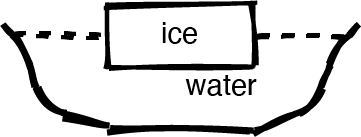
\includegraphics{./img_traning/bathtub.png}
\caption{Bañera y hielo}
\end{figure}

La respuesta correcta es que el nivel se mantiene igual: el hielo desplaza su propio peso en el agua, por lo que llena exactamente el ``agujero'' que ha hecho cuando se derrite. Averiguar por qué ayuda a las personas a construir un modelo de la relación entre peso, volumen y densidad {[}Epst2002{]}.

Describa otra evaluación formativa que haya visto o utilizado que requiera que las personas piensen detenidamente e identifiquen defectos en su razonamiento. Cuando haya terminado, explique su ejemplo a un compañero y dele comentarios sobre el suyo.

\hypertarget{una-progresiuxf3n-diferente-individual-15}{%
\subsection{Una progresión diferente (individual / 15)}\label{una-progresiuxf3n-diferente-individual-15}}

El modelo novato-competente-experto de desarrollo de habilidades a veces se llama modelo Dreyfus. Otra progresión comúnmente utilizada son las cuatro etapas de competencia:

\textbf{Incompetencia inconsciente:}
la persona no sabe lo que no sabe.

\textbf{Incompetencia consciente:}
la persona se da cuenta de que no sabe algo.

\textbf{Competencia consciente:}
la persona ha aprendido cómo hacer algo, pero solo puede hacerlo mientras se concentra y aún puede necesitar dividir las cosas en pasos.

\textbf{Competencia inconsciente:}
la habilidad se ha convertido en una segunda naturaleza y la persona puede hacerlo reflexivamente.

Identifique un tema donde se encuentra en cada nivel. ¿En qué nivel se encuentran la mayoría de sus alumnos en la materia que enseña con más frecuencia? ¿A qué nivel estás tratando de llegar? ¿Cómo se relacionan estas cuatro etapas con la clasificación novato-competente-experto?

\hypertarget{quuxe9-tipo-de-computaciuxf3n-individual-10}{%
\subsection{¿Qué tipo de computación? (individual / 10)}\label{quuxe9-tipo-de-computaciuxf3n-individual-10}}

{[}Tedr2008{]} resume tres tradiciones en informática:

\textbf{Matemático:}
Los programas son la encarnación de algoritmos. Son correctos o incorrectos, así como más o menos eficientes.

\textbf{Científico:}
Los programas son modelos más o menos precisos de procesos de información que pueden estudiarse utilizando el método científico.

\textbf{Ingenieria:}
Los programas son objetos construidos como represas y aviones, y son más o menos efectivos y confiables.

¿Cuál de estos coincide mejor con su modelo mental de computación? Si ninguno de ellos lo hace, ¿qué modelo tienes?

\hypertarget{explicando-por-quuxe9-no-pares-5}{%
\subsection{Explicando por qué no (pares / 5)}\label{explicando-por-quuxe9-no-pares-5}}

Uno de sus alumnos piensa que hay algún tipo de diferencia entre el texto que escriben carácter por carácter y el texto idéntico que copian y pegan. Piensa en una razón por la que podrían creer esto o algo que podría haberles sucedido para darles esta impresión, luego finge ser ese aprendiz mientras tu pareja explica por qué este no es el caso. Intercambie roles e intente nuevamente.

\hypertarget{su-modelo-ahora-toda-la-clase-5}{%
\subsection{Su modelo ahora (toda la clase / 5)}\label{su-modelo-ahora-toda-la-clase-5}}

Como clase, cree una lista de los elementos clave de su modelo mental de aprendizaje. ¿Cuáles son la media docena de conceptos más importantes y cómo se relacionan?

\hypertarget{sus-muxe1quinas-nocionales-grupos-pequeuxf1os-20}{%
\subsection{Sus máquinas nocionales (grupos pequeños / 20)}\label{sus-muxe1quinas-nocionales-grupos-pequeuxf1os-20}}

Trabajando en grupos pequeños, escriba una descripción de la máquina nocional que desea que los alumnos usen para comprender cómo funcionan sus programas. ¿En qué se diferencia una máquina nocional para un lenguaje basado en bloques como Scratch de la de Python? ¿Qué pasa con una máquina nocional para hojas de cálculo o para un navegador que interpreta HTML y CSS al representar una página web?

\hypertarget{disfrutando-sin-aprender-individual-5}{%
\subsection{Disfrutando sin aprender (individual / 5)}\label{disfrutando-sin-aprender-individual-5}}

Múltiples estudios han demostrado que las evaluaciones de enseñanza no se correlacionan con los resultados del aprendizaje {[}Star2014, Uttl2017{]}, es decir, qué tan bien los estudiantes califican un curso no predice cuánto recuerdan. ¿Alguna vez has disfrutado de una clase de la que realmente no aprendiste nada? Si es así, ¿qué lo hizo agradable?

\hypertarget{resumen}{%
\section{Resumen}\label{resumen}}

\begin{figure}
\centering
\includegraphics{./img_traning/conceptmap-mental-models.svg}
\caption{Modelo mental}
\end{figure}

\begin{figure}
\centering
\includegraphics{./img_traning/conceptmap-assessment.svg}
\caption{Efaluación formativa}
\end{figure}

\hypertarget{applications}{%
\chapter{Applications}\label{applications}}

Some \emph{significant} applications are demonstrated in this chapter.

\hypertarget{example-one}{%
\section{Example one}\label{example-one}}

\hypertarget{example-two}{%
\section{Example two}\label{example-two}}

\hypertarget{final-words}{%
\chapter{Final Words}\label{final-words}}

We have finished a nice book.

\end{document}
